\chapter{Determining ship induced wave height at the beginning of the fore shore} \label{Chp:shipwaves}

To determine the ship induced wave height $H_0$ \unitbrackets{m} at the beginning of the fore shore, the following formula is used (source: Handleiding DIPRO, 1997)

\begin{equation}
H_0 = \alpha_1 h \left ( \frac{s}{h} \right )^{-1/3} Fr^4
\end{equation}

with

\begin{symbollist}
\item[$\alpha_1$] ship dependent coefficient \unitbrackets{-}
\item[$Fr$] Froude number ($Fr$<0.8) \unitbrackets{-}
\item[$h$] water depth (considering a  trapezoidal profile) \unitbrackets{m}
\item[$s$] distance of shore to ship \unitbrackets{m}
\end{symbollist}

The Froude number, a dimensionless quantity indicating the mean flow velocity relative to the speed of free surface waves, is computed as:

\begin{equation}
Fr = \frac{v_s}{\sqrt{g h}}
\end{equation}

with

\begin{symbollist}
\item[$g$] gravity acceleration 9.81 \unitbrackets{m/s\textsuperscript{2}}
\item[$v_s$] ship velocity \unitbrackets{m/s}
\end{symbollist}

The value of the Froude number is limited to 0.8 and \autoref{Tabships} shows the values used for the coefficient $\alpha_1$, with 
\begin{symbollist}
\item[$T_s$]  the draught of the ships \unitbrackets{m}
\end{symbollist}


By using these formulas, the value of $H_0$ can be computed based on the dominant ship type, their velocity and draught, the distance between fairway and shore and the water depth.

\begin{table}[!h]
	\begin{tabular}{ll}
		Ship type & $\alpha_1$ \\ \hline
		Push barge & 0.5 \\
		RHK ship / Motorship & 0.28 $T_s^\text{1.25}$ \\
		Towboat & 1.0 \\ \hline
	\end{tabular}
	\caption{Ship-types supported by D-Fast Bank Erosion, with $T_s$ \unitbrackets{m} the draught of the ships}
	\label{Tabships}
\end{table}

\clearpage
To prevent wave load on smaller channels far from the main channel, the wave height is smoothly reduced to zero from distance $s_1$ to $s_0$ from the fairway.
This is accomplished by multiplying $H_0$ with the following function:

\begin{equation}
f(s) = \left \{ \begin{matrix}
1 & 0 < s < s_1 \\
\cos \left ( \frac{s - s_1}{s_0 - s_1} \pi \right ) & s_1 < s < s_0 \\
0 & s > s_0
\end{matrix} \right .
\end{equation}

The value for $s_0$ will be in the order of 150 - 200 m and for  the following relation is used: $s_1 = s_0 - 50$.
In \autoref{Fig5.1} the wave height $H_0$ as function of the distance from the fairway $s$ is depicted for various values of the water depth $h$ for a moter ship with a draught of 1.2 m with a relative velocity of $v_s = 6$ m/s.
The wave height is reduced to zero between $s_1 = 100$ m and $s_0 = 150$ m.

\begin{figure}[!hb]
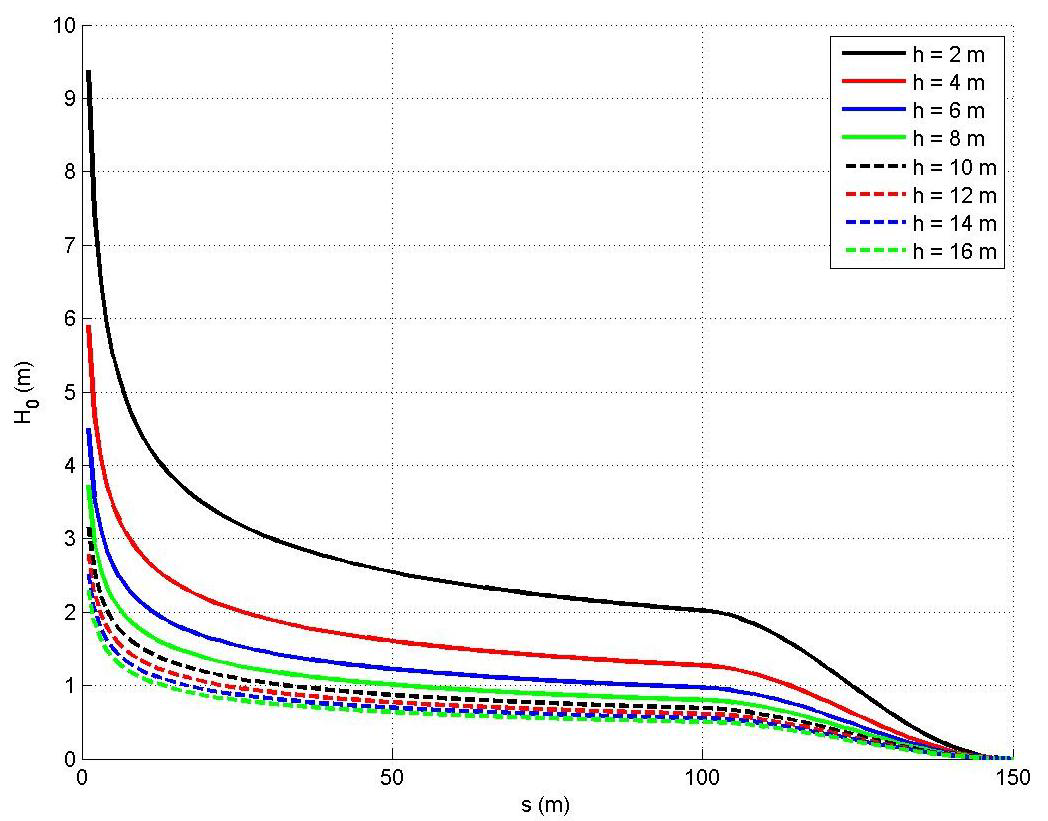
\includegraphics[width=\textwidth]{figures/Fig5-1.png}
\caption{Wave height as function from the distance from the fairway for different values of the water depth.}
\label{Fig5.1}
\end{figure}
